
\subsection{IMPLEMENTACIÓN DE LOS CLIENTES}

Un cliente puede ser definido como un equipo o software que se conecta a un
servidor para obtener un beneficio, sea por poder de computo, para obtener
una información dada o comunicarse con un programa que se ejecuta en el lado
del servidor. Siguiendo esta definición, se crearon 2 clientes, uno para
facilitar la inserción de datos en la simulación del sensor, y el cliente Web,
el cual permite manejar el análisis y la monitorización de los sensores.

\subsubsection{Cliente de Sensorica}

Este fue elaborado en Go para facilitar la interconexión con el servidor y
de igual forma aprovechar el paralelismo y la multiplataforma que el
lenguaje ofrece. Se puede subdividir en 3 acciones fundamentales:

\begin{itemize}
    \item GUI: Es la interfaz gráfica de usuario, utiliza el Framework Fyne por
        facilidades
        de diseño y es una ventana que permite ingresar datos equivalentes
        a las características del motor y conectar con el servidor (además de
        especificar en qué dirección está el motor), y posee una ventana de
        \textbf{log}  en la cual se comunica al usuario acciones como la conexión exitosa y
        el envío de información al servidor. esta puede ser vista
        en la figura \ref{img:fyne} y como se observa, permite especificar:
        \begin{enumerate}
            \item Dirección Ip: Lugar a conectar.
            \item Id Motor: Identificador único del motor.
            \item Potencia: Información adicional, opcional.
            \item Nivel de daño: numero entre 1 y 10 que determina los posibles
                valores del modelo.
            \item Información: Información adicional, pensado para comentarios,
                opcional.
            \item Sensores: lista de 1 a 5 posibles sensores, que representan
                los identificadores únicos que tienen los sensores asociados
                al motor.
        \end{enumerate}

        Cabe resaltar que a ser una GUI es el proceso principal, las demás
        tareas son realizadas de forma paralela.

    \item Conexión al servidor: Es un protocolo que ocurre cada vez que se presiona
        el botón de \textbf{conectar}, se encarga de intercambiar información con el servidor
        para poder conectarse (bajo el protocolo Https) y envía los datos de
        qué motor se va a conectar (simular) y qué sensores tiene asociados, espera
        una aprobación de conexión (para que no exista un motor con el mismo id enviando
        información), obtiene las características especificadas en la GUI y
        comienza un proceso de envió-recibo de información.
        Este es un proceso
        que se ejecuta paralelamente a la GUI y se inicia cada vez que se
        presiona el botón de \textbf{conectar}, Si había un proceso previo y se vuelve a
        presionar \textbf{conectar} finaliza el anterior y comienza uno nuevo.

    \item Comunicación con el servidor: Es un proceso de envió bidireccional
        de información, esta rutina se inicia cuando la conexión al servidor
        es completada exitosamente y se subdivide en 3 procesos que, a su
        vez, corren paralelamente (se toma el proceso de conexión al servidor
        y se crean 2 hijos para un total de 4 procesos paralelizados si se
        incluye la GUI). Estos procesos son:

        \begin{enumerate}
            \item \textbf{timer}, Es un proceso que se encarga de cronometrar
                cada cuánto
                se va a mandar un mensaje de información con los datos
                correspondientes a una medición normal al servidor.

            \item \textbf{listen}, Es un proceso que se encarga de verificar si
                hay una
                solicitud de información, ya sea del subproceso \textbf{imer} (como un
                mensaje normal) o del servidor para solicitar información de la
                vista exhaustiva (la cantidad de información enviada es sustancialmente
                diferente) o para la terminación del proceso e informa a \textbf{handler}
                qué se debe hacer.

            \item \textbf{handler}, Se encarga de realizar la tarea pedida por \textbf{listen},
                al enviar la información solicitada al servidor, enviando 2 mensajes;
                uno con el tipo de información que se envía y otro con la información.
                Esto fue establecido como una especie de protocolo para dar mayor
                seguridad y a la vez facilitar el intercambio de información con
                el servidor.
        \end{enumerate}

        Cabe resaltar que estos procesos son asíncronos y no sufren prelaciones
        entre ellos.
\end{itemize}

\begin{center}
    \begin{figure}[H]
		\centering
        \caption{GUI del cliente de sensorica}
        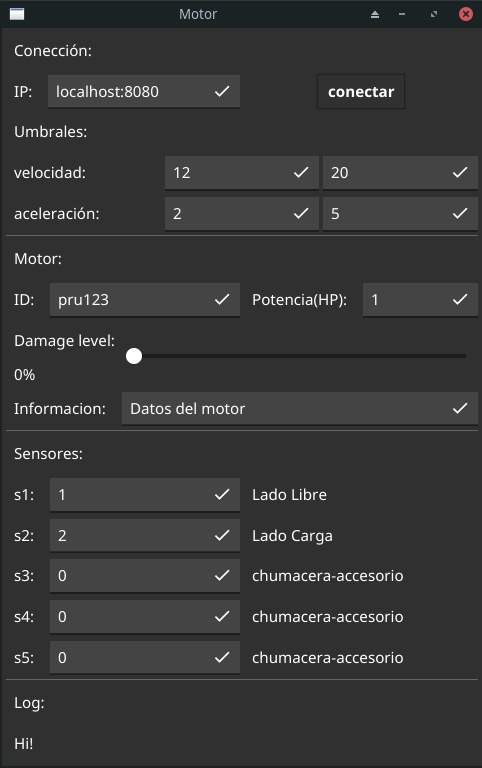
\includegraphics[width=10cm]{clients/ClienteSensoricaSinConectar.png}

        Interfaz de usuario para la conexion del cliente de sensorica. \label{img:fyne}
	\end{figure}
\end{center}

\subsubsection{Cliente Web}

Este cliente es el mas conocido, ya que es el que permite que se muestre la
información en el navegador Web. Está constituido por las vistas general,
específica y exhaustiva, cada una de ellas representa una página Web separada y
todas fueron construidas utilizando el Framework de JavaScript \textbf{React}
y con HTML específicamente un Template de Django y CSS para dar estructura
básica y estilo respectivamente.

Se optó por utilizar un
estilo multi páginas con renderizado de lado servidor (específicamente del
servidor Web) por la necesidad de los cálculos avanzados y gráficas que
se deben realizar, además de los llamados importantes e interconexiones con la
API del servidor de Go y de las BBDD. Esto difiere con el paradigma tradicional de
React (monopágina de renderizado en servidor) pero permite optimizar recursos y
facilita expansiones a futuro.

Su estructura viene dada por las 3 páginas o sub aplicaciones que permiten:

\begin{itemize}
    \item General: conocer el estado general de un grupo de motores, indicando
        en código de colores (verde, amarillo, rojo) el nivel de daño que posee
        un motor. Este nivel es determinado por las muestras mas actuales de
        la información del motor y unos valores parámetros proporcionados en
        conjunto con los datos de los cuales se elaboró el modelo estadístico.

        Cabe resaltar que estos valores son una extrapolación empírica de la
        vibración en una planta específica, es configurable y puede variar dadas
        las características propias de cada instalación. Esto es debido a que
        las bases utilizadas en la instalación, los soportes, entre otros factores
        \textbf{causados por ignorar las normas de instalación} afectan las medidas.

    \item Específica:  permite el estudio del estado de un motor específico,
        es enviado el parámetro que lo identifica en el Url, al servidor.
        Permite observar
        una gráfica histórica y una tabla exportable a excel de sus características y
        evolución en el tiempo, siempre y cuando se tenga medición de ese periodo
        en la base de datos, asimismo permite solicitar la vista exhaustiva del
        mismo motor si es requerido un nivel mayor de análisis.

    \item Exhaustiva: esta vista incluye todo lo anterior de la vista específica,
        con la diferencia de que permite regresar al menú general en vez de hacer
        una vista exhaustiva; además, realiza un análisis en frecuencia
        del estado a tiempo real del motor. Este análisis se puede realizar si
        se tiene acceso en tiempo real con el motor, es decir,
        el servidor de \textbf{sensorica} debe tener una conexión con un sensor que se
        encargue de monitorear el respectivo motor permitiéndole así solicitar
        la información necesaria para hacer el análisis.

        Cabe resaltar que esta acción es tratada como una vista aparte ya que
        tiene un peso computacional relativamente alto asociado y, por ende,
        además de consumir recursos tiene una duración de carga de algunos
        segundos que deteriora la experiencia de usuario, por esto
        obtiene solamente por una solicitud explicita.
\end{itemize}




